
%(BEGIN_QUESTION)
% Copyright 2006, Tony R. Kuphaldt, released under the Creative Commons Attribution License (v 1.0)
% This means you may do almost anything with this work of mine, so long as you give me proper credit

How much pressure, in inches of water column, is being applied to this inclined water manometer to create a total displacement of 14 inches along the length of the tubes, inclined at angles of 20$^{o}$ from horizontal?  Assume the base of this manometer is located 24 inches above ground level.

$$\includegraphics[width=15.5cm]{i00168x01.eps}$$

Next, convert this pressure into units of kPa.

\vskip 20pt \vbox{\hrule \hbox{\strut \vrule{} {\bf Suggestions for Socratic discussion} \vrule} \hrule}

\begin{itemize}
\item{} Identify which fundamental principles of science, technology, and/or math apply to each step of your solution to this problem.  In other words, be prepared to explain the reason(s) ``why'' for every step of your solution, rather than merely describing those steps.
\item{} Does inclining a manometer make it more or less sensitive to applied pressure?  Develop a ``thought experiment'' where you could test a manometer to answer this question.
\item{} Is it possible to make a {\it well} version of an inclined manometer so that we need only to read one liquid column?
\item{} What will happen to a manometer if it is exposed to a gas pressure greater than its measurement range?
\item{} Would a {\it micromanometer} be more or less sensitive to applied pressure than this inclined manometer?
\end{itemize}

\underbar{file i00168}
%(END_QUESTION)





%(BEGIN_ANSWER)

Applied pressure = 1.193 kPa

%(END_ANSWER)





%(BEGIN_NOTES)

The 24 inch height from ground level is extraneous information, included for the purpose of challenging students to identify whether or not information is relevant to solving a particular problem.

\vskip 10pt

The diagonal displacement of 14 inches equates to a vertical displacement of only 4.7883 inches, as described by the {\it sine} function:

$${h \over 14} = \sin 20$$

$$h = 14 \sin 20$$

$$h = 4.7883$$

Therefore, the applied pressure is equal to 4.7883 inches of water column ("W.C).

\vskip 10pt

Approximating certain trigonometric functions from memory is not as difficult as one might think.  Consider the following ``easy angles'' for the sine and cosine functions:

$$\sin 0^o = 0 = \cos 90^o$$

$$\sin 30^o = 0.5 = \cos 60^o$$

$$\sin 45^o = {\sqrt{2} \over 2} = \cos 45^o$$

$$\sin 60^o = {\sqrt{3} \over 2} = \cos 30^o$$

$$\sin 90^o = 1 = \cos 0^o$$

These may be made easier to remember by writing the constants a bit differently:

$$\sin 0^o = {\sqrt{0} \over 2} = \cos 90^o$$

$$\sin 30^o = {\sqrt{1} \over 2} = \cos 60^o$$

$$\sin 45^o = {\sqrt{2} \over 2} = \cos 45^o$$

$$\sin 60^o = {\sqrt{3} \over 2} = \cos 30^o$$

$$\sin 90^o = {\sqrt{4} \over 2} = \cos 0^o$$

Much easier, right?

%INDEX% Measurement, pressure: inclined manometer
%INDEX% Mathematics, trigonometry: approximating trig functions from memory

%(END_NOTES)


